\documentclass[a4paper]{article}

%% Language and font encodings
\usepackage[english]{babel}
\usepackage[utf8x]{inputenc}
\usepackage[T1]{fontenc}

%% Sets page size and margins
\usepackage[a4paper,top=3cm,bottom=2cm,left=3cm,right=3cm,marginparwidth=1.75cm]{geometry}

%% Useful packages
\usepackage{algorithm}
\usepackage[noend]{algpseudocode}
\usepackage{amssymb}
\usepackage{amsmath}
\usepackage{graphicx}
\usepackage[colorinlistoftodos]{todonotes}
\usepackage[colorlinks=true, allcolors=blue]{hyperref}
\usepackage{subcaption}

%% NIPS format
\usepackage{nips13submit_e,times}

\author{Yana Hasson}

\begin{document}

\begin{abstract}
Style transfer aims at creating new images that preserve from a sample image the subjective characteristics known as style. The transfer can be considered as successful if the new image clearly preserves the composition of the original image while producing the same visual impression as the image from which we imitate the style. 
With the development of virtual and augmented reality, there is a growing demand for high quality synthesized images that produce either realistic or graphical impressions on the viewer. By providing realistic or style-specific visual results on a finer scale to basically drafted synthesized images, style transfer can significantly enrich the user’s visual experience. Another interest is purely artistic, as it allows to create new images that mimic various painting styles, therefore producing interesting aesthetic results.
One approach of style transfer is directly inspired from texture transfer and aims at mapping patches from the style image to the content image in order to preserve small scale details while trying to produce comparable large scale items.
An inherent problem in this case is therefore the ability to distinguish between object details and style attributes that are of similar size.  
In this paper, we further explore the application of adaptive size patch quilting to style transfer to preserve fine-grained details of the original image that are below the maximal scale of the texture pattern. To do this, we use a quad-tree structure that takes into account both the local homogeneity of the content image and the local ability to be faithfully mapped to the style image. We try to improve upon the original method to allow for more fine-tuning of the splitting. Allowing for more adaptation of the quad-tree splitting for the transfer task given a specific style-content pair of images improved the final visual result. We also propose to operate the regularization of the patch selection at the same time as the splitting and quilting occurs, using the same rules for the splitting as for the patch selection. This allows us to have a splitting that takes into account all the constraints of the problem.
\end{abstract}

\section{Introduction}

In a style transfer task, two uncorrelated images are used to produce a new one. A 'content' image contains a layout of recognizable items, which form the composition of the scene. A second 'style' image serves as an example of the general visual impression that we want the final image to convey.
One of the difficulties is that the style image usually depicts recognizable items beyond the specific style. The extraction of style attributes from the style image must therefore be conducted carefully in order to capture the style's characteristics independently from composition of the style image.

Although style refers to an immediate visual perception, it is non-trivial to formalize. A first approximation is to consider style as the lower-scale details of the image that are independent of the content, and therefore found repeatedly in places that correspond to different items of the image. 
For instance, it can be the aspect of the brush-stroke or a pencil, or larger-scale patterns that are consistently repeated by the painter across the painting.

In this context, texture-transfer can be seen as a specific case of style-transfer where the style image does not contain any recognizable items and is therefore restricted to texture details. As texture transfer is a problem that has been extensively studied, style transfer methods can directly benefit from the methods that were developed for this purpose.

For texture-transfer, various approaches have produced visually satisfying results.

Methods that tried to extensively capture the statistics of the underlying stochastic process have been rapidly rejected because of the important computational effort involved by such methods. The first visually interesting results in texture transfer derive from techniques where the new image is grown one pixel at the time. 

Wei and Levoy ~\cite{wei-levoy} considered the entire possible span of pixels' neighborhoods from the texture image to grow textures one pixel at the time, selecting the most likely color values given the already synthesized neighborhood, which is named the causal neighborhood. They also introduced a multi-scale pyramidal synthesis process which allowed high-frequency details to be coherent with low-frequency ones. By synthesizing images forming a pyramid from a coarse scale to finer ones, considering the previously synthesized at various coarse scales, they achieved state of the art results for texture synthesis. They therefore created an algorithm that allowed to create larger samples of a texture from an original small sample, thus opening the way to texture transfer techniques where textures were mapped pixel by pixel from a small samples to larger example images.

The described method has the drawback of being computationally expensive and sometimes gets stuck in local minima, synthesizing always the same sequence of pixels and therefore failing to reconstruct complex patterns by producing 'garbage'.
The second limitation is solved by Ashikhmin ~\cite{natural-textures} which also synthesizes the pixels one by one in scanline order. The new pixel is chosen from a small list of candidates by minimizing neighborhood distances. The candidates are selected by looking at the pixels from the texture image that were mapped to the causal neighborhood of the currently synthesized pixel. Among those neighbors, the chosen pixel is the one that has the same relative positioning to the causal pixel and for which the neighborhood distance is minimal. Preserving the relative positioning of the candidate to the neighbor pixel in the final image is effectively equivalent to growing patches of irregular shapes. This method faithfully transfers the texture in the specific case of textures composed of small irregular shapes of various small sizes, but produces sharp edges between two synthesized patches which makes this method inadequate for general texture.  Ashikhmin ~\cite{fasttransfer} also introduced a variant that performs texture transfer onto simple flat color drawings, getting closer to our more complex objective of transferring styles. This method jointly minimizes the distance of the causal neighborhood to the texture sample image and the complementary part of the neighborhood to the color image. The algorithm therefore overwrites the color image with pixels from the texture sample by preserving both a local coherency between already synthesized pixels and a consistency with the color image neighborhood.

A somewhat different approach is taken in  ~\cite{quilting}, as it introduces the idea of mapping square image patches sampled from the texture image to the content image by minimizing the intensity distances. This approach therefore does not rely on individual pixel synthesis and can be computationally more efficient. In this case, the quality of the transfer depends strongly on the chosen size of the patch, which is taken as a rule of thumb as the order of magnitude of the largest visible patterns of the texture. Using this patch size focuses on preserving the full complexity of the pattern, but often at the expense of the finer details of the original image. 
As patches are used, borders have to be blended in order to avoid introducing a visually striking square grid on the final image. Efros and Freeman \cite{quilting} therefore performs the image quilting with an overlap and operate a boundary cut in order to attenuate the square's borders. The borders are made uneven in a way that maximizes visual coherency, operating the cut where the pixels are most similar in the overlapping region.
Visually, this method often outperforms methods that focus on individual pixels at a lesser computational price.
In this article, although style transfer is not explicitly mentioned, the method could be directly applied to this task. In this case, the same shortcomings as the ones for texture transfer would apply because of the fixed choice of the patch size.

A new method presented by Frigo et al ~\cite{adaptative-quilting} explicitely focuses on style transfer and tries to alleviate the issue of a fixed-size patch by introducing an adaptative quilting technique. Instead of having a fixed path size, a quadtree structure is constructed before the quilting is performed. Starting from a square image, successive splits are made, each split dividing a square block into four equal smaller squares. The quadtree construction takes into account two factors in order to decide whether a finer split should occur. The first parameter considered is the local homogeneity of the content image, which is computed by the mean of the pixel variance of the current square block of the content image. Favoring local homogeneity encourages splitting if the current square is irregular, and is therefore likely to contain relevant content details.  The second parameter is the local proximity to the style image, which is accounted for by the minimal squared pixel distance to same-size patches of the style image. This way, splitting occurs if no satisfying match for the current patch is found in the style image. As different patch sizes are considered, a normalized patch distance d is considered by dividing the sum of square of pixel distances over the patch by the number of pixels in the given block. The quadtree splitting also takes into account a minimal and a maximal patch size, ${\gamma_{min}}$ and ${\gamma_{max}}$ which enables some balancing between the maximal size of exact copying of the original image, and the computational intensiveness. During the splitting, a set of optimal candidates from the style image are chosen from the style image using a constrained k-nn to provide a diversity among the selected patches. At the final stage a label is assigned to each block of the final quadtree by taking into account both the closeness to the content block and the visual continuity between style patches in order to try to provide the best visual result. 

Building upon this work, we tried to improve the obtained result by addressing two aspects of the quadtree quilting method. A first step is to separate the contribution of the local inhomogeneity and the contribution of the distance to the style patches. This separation would allow us to dissociate and finetune for a given image the persistence of the details and the closeness of the mapping to the style image. We also decided to replace the constrained k-nn, choosing a single label at split and quilting time and trying to compensate for the potential loss of continuity by operating a boundary cut as presented by Efros and Freeman ~\cite{quilting}. We therefore intend to produce an efficient merging of the patches in cases where the two patches that are mapped as neighbors are not as close as in the examples provided by the original quadtree quilting method, and the bilinear blending therefore proves to be unsatisfying. On the other hand, to account for the effort to limit repetition of similar patches close by, we will take into account the distance between blocks that have been mapped to the same patch.  

We will then compare our results to recent state of the art style transfer results that were introduced by Gatys and al ~\cite{neuralstyle} using convolutional neural networks. This method minimizes a weighted loss of composed of two terms, one that is associated to the style of an image, and the other that is associated to the content of another image. The goal of the method is then to find an image that minimizes this loss, effectively producing an image that, to some extent, imitates the style of the first image while preserving the content of the second one.
The style loss is expressed as a weighted sum over several layers. It is taken to be the sum of square distances of the correlations between activations for different filters across all possible filter positions. The content loss is simply the sum of squared differences for a given convolutional layer between the activations for two different images. 
By jointly minimizing these two losses on various layers, Gatys and all manage to transfer styles from one image to another. The choice of the layers on which they choose to apply the content loss determines to some extent the minimal scale at which the content will be preserved, with the choice of earlier layers providing finer details.



\section{Original adaptative quilting}

The decision for a given square patch to be split can be summed up according to ~\cite{adaptative-quilting}  by the following condition :

\[ C(p_{x_i}, p_{y_i}) = ((\sigma_i + d(p_{x_i}, p_{y_i})) > \omega \  and  \ \tau_i  > \gamma_{min}) \ or \ (\tau_i < \gamma_{max}) \] 


Where ${d(p_{x_i}, p_{y_i}))}$ is the distance of the ${i^{th}}$ patch of the content image to the closest patch ${p_{y_i}}$ from the style image. ${\tau_i}$ being the current patch scale, the size in pixels of the side of the square patches.

${p_{y_i}}$ is therefore the patch of the style image that minimizes the following distance :

\[d(p_{x_i}, p_{y}) = \frac{||p_{x_i}-p_y||}{{\tau_i}^2}\] 

Where the square of the chosen norm that is the sum of square differences for each color channels. 

The variance term is the standard deviation of pixel illumination.

\[\sigma_i = \sqrt{Var(p_{x_i})}\]

\[\sigma_i  = \sqrt{\sum_{x \in p_{x_i}}(I_{x} - I_m)^2}\]

where $I_m$ is the mean pixel intensity, $I_x$ is the illumination at pixel x, x belonging to the patch $p_{x_i}$

Three parameters are left for the user of the algorithm to tune. ${\omega}$, which triggers a split if the sum of the contributions of the local variance and of the distance to the style image are too large, and the minimum and maximum patch sizes $\gamma_{min}$ and $\gamma_{max}$.

For the leaf blocks of the quadtree (blocks which have failed the condition C and have therefore reached their final size), k-nearest neighbors from the style image are computed. The k-nn algorithm is constrained such as to limit the number of direct neighbors from the style labels among the candidates. The constraint enforces a minimal distance between two candidate patches.

Once all candidate patches are computed for each of the leaf blocks, the final stitching occurs, trying to optimize a probability density that considers for each patch a data fidelity term and a pairwise compatibility term.

The term we want to maximize over the candidate label assignments is 

\[P(L)=\frac{1}{Z} \prod_{i}{\Phi(l_i)}\prod_{(i,j \in N)}{\Psi(l_i, l_j)}\]

Where i describes the leaf blocks’ indexes, and N is the ensemble of direct neighbors in the quadtree knowing that two blocks are considered as direct neighbors if one of their edges is at least partly shared.

$\Phi$ is the data fidelity term, which takes into account the distance between the $i^th$ block and the candidate label.



\[\Phi(l_i) = exp(-\lambda_d*d(p^{imcontent}_{x_i}, p^{imstyle}{l_i} ))\]

$\Psi$ is the pairwise compatibility term, 

\[\Psi(l_i, l_j) = exp(-\lambda_s*d(\hat{p}^{imstyle}_{l_i}, \hat{p}^{imstyle}{l_j} ) + \lambda_r *|l_i-l_j|^2))\]

$\hat{p}^{imstyle}_{l_i} and \hat{p}^{imstyle}_{l_j}$ are the overlapping parts of two patches that have been grown in order to produce some overlap around the shared edge. This term aims at encouraging smoothness at the edges as it enforces similarity between the patches around their shared limits. The second term penalizes label repetition, as $\Psi$ decreases if the two labels are very different.
$|l_i - l_j|^2$ is the square of the distance between the two patches from the style image. We can notice that by penalizing label repetition with this distance, there is also a penalization for close neighbors, therefore it is less likely that direct neighbors in the style image will be mapped to direct neighbors in the final image. This might be an unwanted side effect, as keeping neighbors together would increase perceived visual coherence.

As patches are stitched together in this method, the issue of apparent edges has to be addressed. In the original paper, a simple bilinear blending is applied, producing satisfying results in the presented final images. Although bilinear blending is known to have limited smoothing capacities for images, as the regularization emphasizes similarity over overlapping areas, the final bilinear blending is often enough to suppress visible edges.




\section{Improvements of quadtree style transfer}


\subsection{Disentangling of variance and style proximity}

To improve upon the method presented by Frigo and al ~\cite{adaptative-quilting}, we started by reimplementing the quadtree splitting algorithm as described in the original article in order to apply it to a new selection of style and content images. 

Our first observation was that using a quadtree structure as described by Frigo and al forces the original content image and the final image to be square, and even more restrictively, the finale size S of the image must be the product of ${\gamma_{min}}$ and ${2^n}$ where n $\in$ $\mathbb{R}$.
We therefore have ${S = \gamma_{min}*2^n}$, and n is the maximum depth of splits that will occur during the quadtree construction.

We will therefore work exclusively with square images that respect this size constraint, cropping and resizing the original content images when needed. 

Starting with the square image, we recursively split each square into four squares until we reach the maximum size for a split ${\gamma_{max}}$. Once we've reached this block size, splits only occur if the condition for a split is satisfied, and the minimal split size ${\gamma_{min}}$ hasn't yet been reached.

To each square that has reached its final size in the content image, we want to assign a label that corresponds to a patch of the same size in the style image.

Implementing the original algorithm revealed an intrinsic limitation of the condition that is evaluated to determine whether a split to occur. By having a single parameter, ${\omega}$ that accounts both for the local homogeneity and the local distance to the style image, for some images, it is difficult to find a good compromise between the two constraints. 
More specifically, we observed that both terms as well as their relative importance could vary a lot from a problem to another.
In the case where the image is highly locally contrasted, for a black and white landscape picture for instance, the variance term was sometimes always largely dominant over the distance one. Therefore, there was no possibility to improve the fidelity of the mapping without producing a uniformly fine-split quadtree on the largest part of the final image.
The opposite situation could also occur, although less often as the variance tended to have both a higher value and variation over the blocks. In the case where the content image and the style image were very dissimilar, for instance if the color tones of the two images would differ greatly, trying to further constrain the scale of the reproduced details would be limited by the closeness term, and a thin splitting would occur in roughly homogeneous regions of the original image.


To deal with those cases, we decided to separate the contributions of the two terms. A split therefore occurs as long as the minimal size hasn't been reached if one of the two constraints, the local homogeneity or the closeness to the style patches is violated.

The new condition that we implemented was therefore:



\[ C(p_{x_i}, p_{y_i}) =  (((\sigma_i  > \omega_{var}) \ or \ (d(p_{x_i}, p_{y_i}) )\ > \omega_{dist}) \  and  \ \tau_i  > \gamma_{min}) \ or \ (\tau_i < \gamma_{max}) \] 

Which can also be written 

\[ C(p_{x_i}, Patches) =  (((\sigma_i  > \omega_{var}) \ or \ (d(p_{x_i}, Patches) )\ > \omega_{dist}) \  and  \ \tau_i  > \gamma_{min}) \ or \ (\tau_i < \gamma_{max}) \] 

Where $(d(p_{x_i}, Patches) )$ is the distance from the the block $p_{x_i}$ to the closest item from $Patches$ which represents all the extracted patches from the style image that have the same size as $p_{x_i}$. 

This rule allows us to control more precisely the splitting for a given image by balancing the two constraints independently to fit our specific needs.

On a specific example with large patch variance variation as in \ref{fig:splits-various-thres-sophie} we can see that for a same sum of thresholds, we can finetune the splitting for a given image. In this case, we purposefully chose a style image that was 'distant' from the content image, so that both thresholds are regularly activated in the thresholding.

Here we can see that by decreasing the variance threshold without modifying the sum of thresholds we can control the splitting around the content image details. By lowering the variance threshold to 10, we manage to produce splits around the mouth and the outline of the face, and therefore increase our chances of making the face recognizable in the final image. If we try produce the same effect by controlling the sum of the thresholds only, we can reduce this global threshold enough to produce the same details, but in this case we also produce additional splits in the region of the hair, where almost all splits occur until they reach the minimal splitting size, creating a large uniform zone of fine-grained splitting which letter often fails to faithfully reproduce the style.  


% \begin{figure}[!h]
% \centering
% \begin{subfigure}{.45\textwidth}
%   \centering
%   \includegraphics[width=.9\linewidth]{split-house-34-2.jpg}
%   \caption{\label{fig:split-house-34-2}var > 34 | dist > 2}
% \end{subfigure}
% \begin{subfigure}{.45\textwidth}
%   \centering
%   \includegraphics[width=.9\linewidth]{split-house-30-6.jpg}
%   \caption{\label{fig:split-house-30-6}var > 30 | dist > 6}
% \end{subfigure}
% \begin{subfigure}{.45\textwidth}
%   \centering
%   \includegraphics[width=.9\linewidth]{split-house-36.jpg}
%   \caption{\label{fig:split-house-36}var + dist > 36}
% \end{subfigure}
% \caption{Quadtree splits for various thresholds }
% \label{fig:splits-various-thres}
% \end{figure}

\begin{figure}[!h]
\centering
\begin{subfigure}{.32\textwidth}
  \centering
  \includegraphics[width=1\linewidth]{sophie-frigo-split-15.png}
  \caption{\label{fig:sophie-frigo-split-15}var + dist > 15 }
\end{subfigure}
\begin{subfigure}{.32\textwidth}
  \centering
  \includegraphics[width=1\linewidth]{sophie-my-split-10-5-split.png}
  \caption{\label{fig:sophie-my-split-10-5-split}var > 10 | dist > 5}
\end{subfigure}
\begin{subfigure}{.32\textwidth}
  \centering
  \includegraphics[width=1\linewidth]{sophie-frigo-split-10.png}
  \caption{\label{fig:sophie-frigo-split-10}var + dist > 10}
\end{subfigure}
\caption{Quadtree splits for various thresholds }
\label{fig:splits-various-thres-sophie}
\end{figure}

\subsection{Implementation details}

The implemented algorithm for the splitting is close to the the original one, although the condition for the split is different.

\begin{algorithm}
\caption{Split and match algorithm}\label{quadtree-algo}
\begin{algorithmic}[1]
\Statex \textbf{inputs} Images : imcontent, imstyle; Thresholds : $\omega_{var}, \omega_{dist}; Limit sizes : \gamma_{min}, \gamma_{max}$
\Statex \textbf{outputs} Set of blocks : R=$\{R_i\}_{i=1,n}^n$; Assigned labels : L=$\{L_i\}_{i=1,n}^n$
\Statex Initialization : $R=regionSplit(imcontent, gamma_{max})$
\Statex $\gamma = \gamma_{max}$ 
\Statex \textbf{while} $\gamma>= \gamma_{min}$ \textbf{do}
\Statex ~~~~patches = getPatches(imstyle, $\gamma$)
\Statex ~~~~\textbf{for} $R_i \in R$ \textbf{do} \textbf{where} $size(R_i)=\gamma$
\Statex ~~~~~~~~$\sigma_i = \sqrt{var(R_i)}$
\Statex ~~~~~~~~\textbf{if} $C(R_i, patches)$ 
\Statex ~~~~~~~~~~~~Split Ri into four
\Statex ~~~~~~~~~~~~$R = \{R$ \textbackslash $R_i\} U \{R_i^1, R_i^2, R_i^3, R_i^4\}$ 
\Statex ~~~~~~~~\textbf{else if}
\Statex ~~~~~~~~~~~~$L_i = p^{imstyle}_{[(argmin_{j}(dist(Ri,patches[j]))]}$
\Statex ~~~~~~~~\textbf{end if}
\Statex ~~~~\textbf{end for}
\Statex ~~~~$\gamma = \gamma /2$
\Statex \textbf{end while}
\Statex \textbf{return}
\end{algorithmic}
\end{algorithm}

$regionSplit(image, \gamma)$ splits the original image in squares of size $\gamma$ while $getPatches(image, \gamma)$ retrieves a set of patches of size gamma from the given image.

This algorithm outputs the final quad-tree splitting of the original image ($R$), and the labels that map each block to a patch from the style image. The algorithm therefore performs the splitting and mapping operations that strive at operating style transfer. We then have to map the selected style patches to the corresponding region position in the image to obtain the final image. 

Several optimizations were perform in order to reduce the computing time, for instance, the getPatches function is only called in the case where one of the blocks at the given size $\gamma$ passes the threshold test. The distance to the current block is also only computed if the variance threshold is passed, as the variance computation is relatively fast in comparison to the distance computation when the number of patches is large. This is furthermore justified in practice, as the variance threshold is often triggered.

Another important aspect of the algorithm is the sampling of patches from the style image. The initial style image is of a given size, and provides wide possibilities for various patch extraction methods. 
The first one that we implemented was a simple cut without overlap at each size $\gamma$ : the style image was cut into contiguous square patches. 
To augment the number of candidates, we also tried to sample with some overlap between the patches, with a fixed overlap size of $decal$. In this case, at a given patch size $\gamma$ the number of sampled patches for a square style image of size $imageSize$ is $floor(\frac{imageSize-\gamma}{decal})^2$, therefore, the number of patches increases as $1/decal^2$. As the k-nn algorithm has to compute the distance to every single patch, a small $decal$ negatively impacted the performances of the algorithm. On the other hand, when $decal$ is above the current patch size $\gamma$, less patches are sampled then if they were contiguously sampled, which can account for a speed-up of the k-nn search.

Another option would have been to adapt the size of the overlap to $\gamma$ as for instance to produce a constant number of patches at each size.


\subsection{Boundary cut}

Experiments on texture synthesis showed that bilinear blending works well if the boundaries are very similar to one another, but tend to perform poorly if the color or illumination variations are more drastic. One of the improvements of Efros and Freeman which allowed them to produce visually coherent textures was using boundary cuts as depicted in \cite{quilting}. A boundary cut is performed by computing a surface error that measures the distance at each overlapping pixel. Once this surface is computed, the cut is operated smoothly by minimizing the global cut price, which is the sum of the distances for the pixels over which the cut path is drawn. More specifically, in my implementation, we decided (arbitrarily) to cut to the right of the minimal path, as we cannot cut a pixel in the middle, and must therefore choose whether to cut at the right or at the left of the minimal path. We could also have operated a mean on the pixels that correspond the chosen path.

To compute the optimal path, we compute the cumulative errors starting from the last row by adding the current error to the minimal cumulative errors from the previous rows among the three closest cumulative error candidates.


\begin{algorithm}
\caption{Compute cumulative errors}\label{patch-cut-algo}
\begin{algorithmic}[1]
\Statex \textbf{inputs} Overlaps : overlap1, overlap2
\Statex \textbf{outputs} Optimal cut path : path 
\Statex errorSurface = getErrorSurface(overlap1, overlap2)
\Statex cumulativeError(lastRowIndex) = errorSurface(lastRowIndex) 
\Statex \textbf{for} rowIndex from lastRowIndex - 1 to 1 with a step of -1  \textbf{do}
\Statex ~~~~\textbf{for} overlapIndex from 1 to 1 overlapSize \textbf{do}
\Statex ~~~~~~~~cumulativeError(rowIndex, overlapIndex) = min(cumulativeError(rowIndex + 1, overlapIndex -1),cumulativeError(rowIndex + 1, overlapIndex), cumulativeError(rowIndex + 1, overlapIndex + 1)) + errorSurface(rowIndex, overlapIndex)
\Statex ~~~~\textbf{end for}
\Statex \textbf{end for}
\Statex \textbf{return}
\end{algorithmic}
\end{algorithm}


$getErrorSurface(overlap1, overlap2)$ computes the error surface as the sum of square errors over the three color channels between the two overlaps.

Once we have the cumulative errors, we can look at the minimal value on the first row, and find a way back through the minimal cumulative error path. 

For the cutting algorithm, the main parameter is the size of the overlapping area, which for convenience was taken as a multiple of two, such as to allow for the extraction of patches from the style image with a padding of half the size of the overlap in all directions. In practice, a total width of overlap of 4 or 6 provided good results in most cases. The compromise that was considered is the quality of the blending versus the ability to preserve fine-grained details. Increasing the size of the overlapping area allowed for more flexibility in the cut, which provided more potential cut paths, and therefore improved the blending. The downside was that those cuts might discard relevant details of the content which are in the same order of size as the overlap size.  

It is interesting to notice that, having implemented a boundary cut following as presented by Efros and Freeman in ~\cite{quilting}, our method is a generalization of their patch-quilting algorithm for square images. Their square quilting algorithm is almost the same as ours in the specific case where ${\gamma_{min} = \gamma_{max}}$, and therefore the local variance and patch distance are not taken into account. 

\subsection{Regularization}

Running the algorithm without any regularization, we can observe that small repetitive patterns appear, affecting the global quality of the transfer. We observed that this effect mainly comes from the same patch of the style image being mapped to neighbors of the content image, sometimes repeatedly over an entire region.

To avoid this phenomena, the original paper produced several candidates for each block and produced a result minimizing a likelihood that took into account regularization parameters. In our case, we operate the regularization in a different way, at the same time as we operate the splitting and quilting of the final image.

The first consideration we made was that the limitation of patch repetition could be operated for each quadtree dimension separately, as two patches of different sizes are by definition different. The second consideration was that the main visual defect was the exact repetition of a unique patch. We therefore adapted the distance term to take into account the distance between identic patches.

To achieve this, we modified the distance in the following way 
   
\[d(p_{x_i}, p_{y}) = \frac{||p_{x_i}-p_y||}{{\tau_i}^2} + \frac{\lambda}{dist(x_i,x_j)/\tau_i} \] 

Where d is the euclidian distance and $x_j$ is the center of the closest block that has been assigned the label that corresponds to the patch $p_y$ of the style image. In the case where no block has been assigned the candidate label before, the distance of the candidate to the same label in the content image is infinite, and therefore the regularization term equals zero. In this case, the total distance is the same as it was previously defined. Also, setting $\lambda$ to zero is equivalent to using the original distance.

Taking the inverse of the distance allows for large penalization of close duplicates of labels and low penalization of distant ones. 

As measuring the distance for all possible candidates from the style image would be computationally prohibitive, we restricted the computation to a limited set of closest neighbors computed by the k-nn algorithm based purely on the normalized patch distance. This also allowed to avoid the case where a locally irrelevant patch would be selected, because all relevant patches have already been mapped closely. In this case, repetition would probably harm the final result less than an irrelevant patch selection.

In practice, we observed that setting $\lambda$ to 4 and choosing between k=5 closest neighbors produced good results : it avoided strict repetition while having a limited effect on the quality of the mapping as far as the proximity to the original data was concerned.



\begin{figure}[!h]
\centering
\begin{subfigure}{.34\textwidth}
  \centering
  \includegraphics[width=.8\linewidth]{china-house-gogh-not-regularized.png}
  \caption{\label{fig:china-house-gogh-not-regularized}Without regularization}
\end{subfigure}
\begin{subfigure}{.32\textwidth}
  \centering
  \includegraphics[width=.8\linewidth]{china-house-gogh-regularized-4.png}
  \caption{\label{fig:china-house-gogh-regularized-4} lambda = 4, k = 5}
\end{subfigure}
\begin{subfigure}{.32\textwidth}
  \centering
  \includegraphics[width=.8\linewidth]{china-house-gogh-regularized-10-k-10.png}
  \caption{\label{fig:china-house-gogh-regularized-10-k-10} lambda = 10, k = 10}
\end{subfigure}
\begin{subfigure}{.32\textwidth}
  \centering
  \includegraphics[width=.8\linewidth]{first-step.jpg}
  \caption{\label{fig:first-step}Style image}
\end{subfigure}
\begin{subfigure}{.32\textwidth}
  \centering
  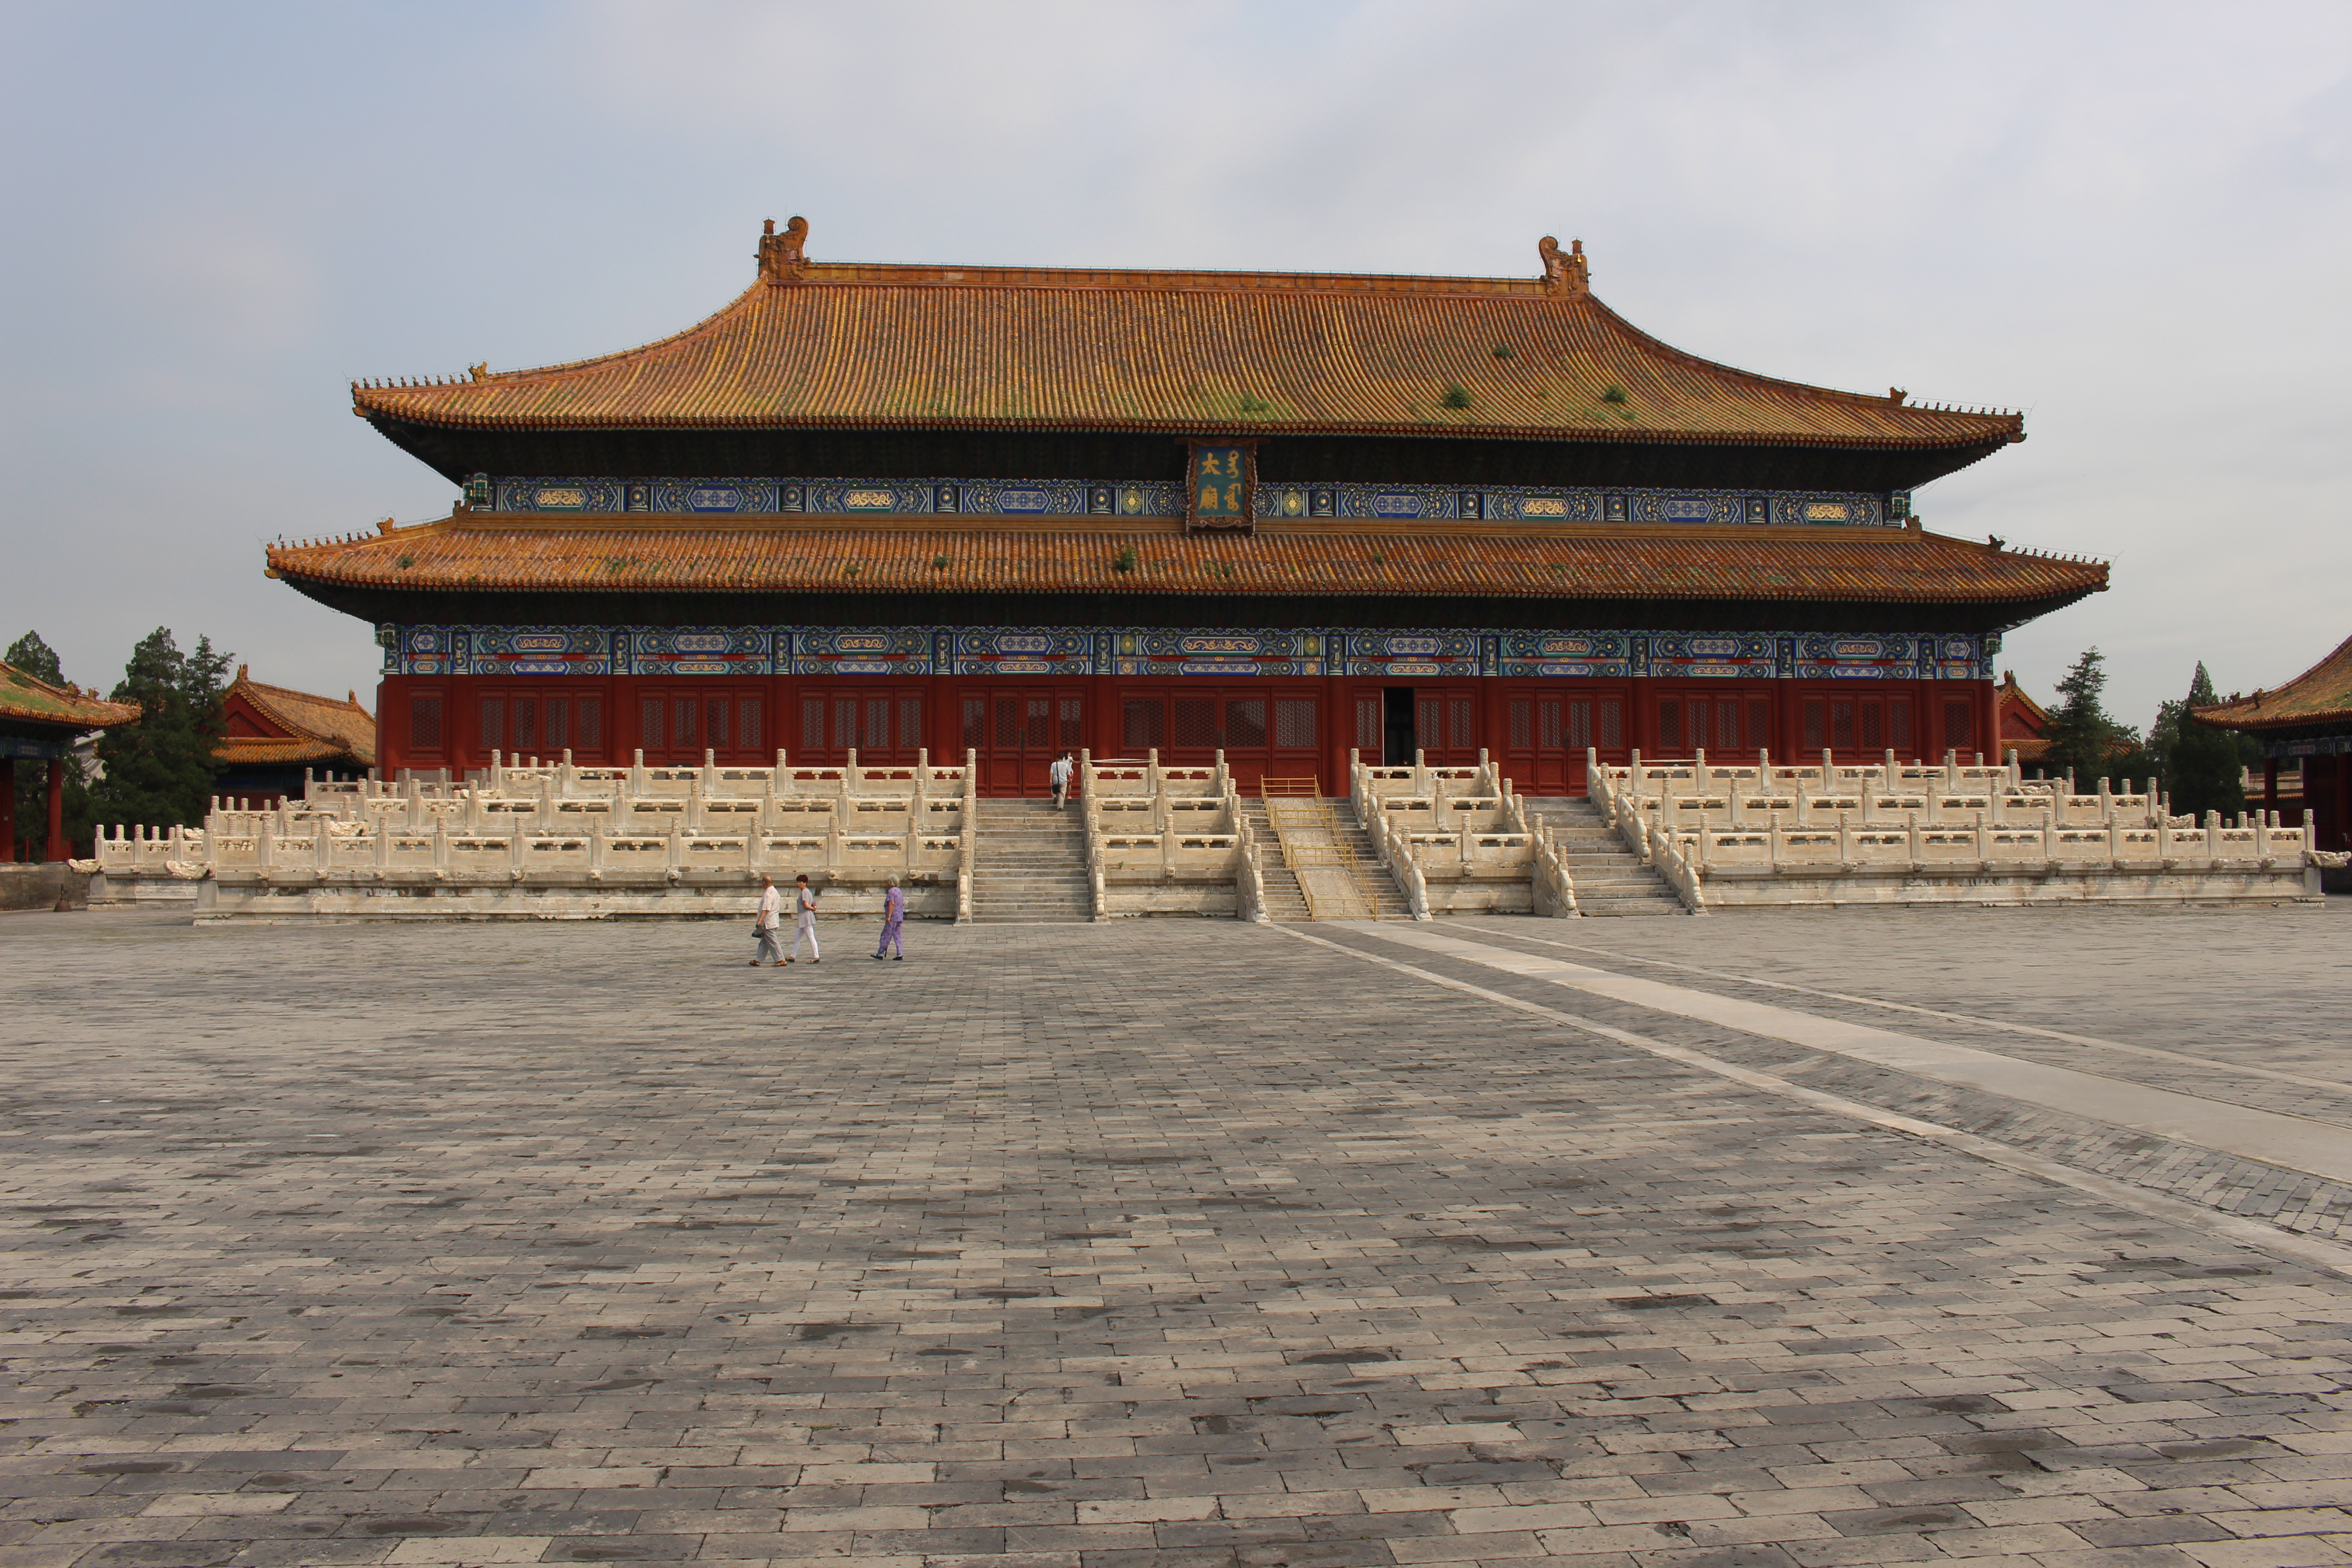
\includegraphics[width=.8\linewidth]{china-archi.jpg}
  \caption{\label{fig:china-archi}Content image}
\end{subfigure}
\caption{Effect of regularization}
\label{fig:regularization-effect}
\end{figure}

We can see looking at \ref{fig:regularization-effect} an example of final images obtained for a content-style pair for various regularization factors and neighbor numbers. We can see that adding distance regularization significantly reduces the visual patch repetition. Between \ref{fig:china-house-gogh-regularized-4} and \ref{fig:china-house-gogh-regularized-10-k-10}  there is an overall diminution of patch repetition. Nevertheless, in the left top part of the sky, we can see the same pattern repeated several times. Since the regularization is operated on the distance only to the exact same patch, and sometimes, there are very similar patches among the candidates. In our current implementation, similar patches are note penalized.

The observed limitation of the regularization becomes stronger when we increase $decal$ and therefore sample a larger number of partially overlapping patches. To take into account the risk of having very similar patches with different labels that might create a visual repetition of patch pattern, instead of taking into account the label of the patches, we could penalize the candidates by taking into account the similarity to their already quilted neighbors, using normalized pixel distance over the style patches for instance.



\subsection{Results}

In \ref{fig:result-comparison}, we present some examples of style transfer operated from pictures of paintings that are freely available for download and use on the website of the Museum of Modern Arts. We chose \textit{View from the artist's window} by Robert Blum, \textit{German Landscape with View towards a Broad Valley} by Fritz Petzholdt and \textit{Study for Portrait of Mrs. Anna E. Little} by Childe Hassam for the variety of the represented styles. The content pictures were also taken to be different from one another. We therefore chose a photo of architectural details of houses, a landscape, and a close-up on a flower.
Those results are presented next to some results that were obtained by running the style transfer through a freely available implementation of the neural style transfer algorithm ~\cite{Johnson2015} that produce similar results in quality to ~\cite{neuralstyle} but with a significant speed-up ~\cite{Johnson2016Perceptual}. The neural style algorithm starts from a random noise image and operates several iterations to minimize the loss that accounts for style consistency and content preservation. In the presented examples, 1000 iterations over the neural network were performed for each image, and in all cases, no significant improvement was observed during the last 300 iterations, which indicates the convergence of the neural transfer algorithm. 

For our method, the patch dimensions were set to $\gamma_{min}=8$, $\gamma_{max}= 64$, the thresholds were set to $\omega_{var} = 18$ $\omega_{dist}=5$. The regularization coefficient was set to $\lambda = 4$, and the $decal$ that regulates the size of the candidate patch set was set to 32. For the cut, each patch was sampled with a padding of 3 pixels, producing a width for overlap region of 6 pixels.


\begin{figure}[!h]
\centering
\textbf{Style images}\par\medskip
\begin{subfigure}{.32\textwidth}
  \centering
  \includegraphics[width=1\linewidth]{blum.jpg}
  \caption{\label{fig:blum}}
\end{subfigure}
\begin{subfigure}{.32\textwidth}
  \centering
  \includegraphics[width=1\linewidth]{fritz.jpg}
  \caption{\label{fig:fritz}}
\end{subfigure}
\begin{subfigure}{.32\textwidth}
  \centering
  \includegraphics[width=.9\linewidth]{pencil-portrait.jpg}
  \caption{\label{fig:pencil-portrait}}
\end{subfigure}
\textbf{Content images}\par\medskip
\begin{subfigure}{.32\textwidth}
  \centering
  \includegraphics[width=.8\linewidth]{square-great.png}
  \caption{\label{fig:square-great}}
\end{subfigure}
\begin{subfigure}{.32\textwidth}
  \centering
  \includegraphics[width=.8\linewidth]{square-flower.png}
  \caption{\label{fig:square-flower}}
\end{subfigure}
\begin{subfigure}{.32\textwidth}
  \centering
  \includegraphics[width=.8\linewidth]{square-houses.png}
  \caption{\label{fig:square-houses}}
\end{subfigure}
% Our images
\textbf{Our results}\par\medskip
\begin{subfigure}{.34\textwidth}
  \centering
  \includegraphics[width=.8\linewidth]{quilt-great-blum2.png}
  \caption{\label{fig:quilt-great-blum}}
\end{subfigure}
\begin{subfigure}{.32\textwidth}
  \centering
  \includegraphics[width=.8\linewidth]{firsflower.jpg}
  \caption{\label{fig:firsflower}}
\end{subfigure}
\begin{subfigure}{.32\textwidth}
  \centering
  \includegraphics[width=.8\linewidth]{quilt-housespenc.png}
  \caption{\label{fig:quilt-housespenc}}
\end{subfigure}
% Neural style image
\textbf{Neural style results}\par\medskip
\begin{subfigure}{.34\textwidth}
  \centering
  \includegraphics[width=.8\linewidth]{square-neural-great.png}
  \caption{\label{fig:square-neural-great}}
\end{subfigure}
\begin{subfigure}{.32\textwidth}
  \centering
  \includegraphics[width=.85\linewidth]{square-neural-flower.png}
  \caption{\label{fig:square-neural-flower}}
\end{subfigure}
\begin{subfigure}{.32\textwidth}
  \centering
  \includegraphics[width=.8\linewidth]{square-neural-houses.png}
  \caption{\label{fig:square-neural-houses}}
\end{subfigure}
\caption{Comparison of style transfer results}
\label{fig:result-comparison}
\end{figure}
\newpage

We observe that both methods fulfill to some extent the style transfer task and that each method has its own strengths and weaknesses.
We can see that for our method, the cuts are still sometimes visible, for instance in the case of the flower \ref{fig:square-flower}. And the patch repetition phenomena is slightly visible in \ref{fig:quilt-housespenc}. In \ref{fig:quilt-great-blum}, we can see an example where content of the style image has been transferred with the style, as we can see that the fence from the original style image \ref{fig:blum} is visible in the sky.
For the neural style transfer, we can observe a slight deformation in \ref{fig:square-neural-houses} that is not linked to a style-related deformation, and in \ref{fig:square-neural-great} we observe that the painting texture was poorly transferred on the sky, leaving it very similar to the original image, although the rest of the image was successfully transformed.


\begin{figure}[!h]
\centering
\begin{subfigure}{.32\textwidth}
  \centering
  \includegraphics[width=.8\linewidth]{impressionist-original.jpg}
  \caption{\label{fig:impressionist-original} Style image}
\end{subfigure}
\begin{subfigure}{.32\textwidth}
  \centering
  \includegraphics[width=.9\linewidth]{frigo-al.jpg}
  \caption{\label{fig:frigo-al} Original quadtree split and matching}
\end{subfigure}
\begin{subfigure}{.34\textwidth}
  \centering
  \includegraphics[width=.9\linewidth]{fuji-original.jpg}
  \caption{\label{fig:fuji-original}Content image}
\end{subfigure}
\begin{subfigure}{.32\textwidth}
  \centering
  \includegraphics[width=.9\linewidth]{our-fuji.png}
  \caption{\label{fig:our-fuji}Our method}
\end{subfigure}
\caption{Comparison with original method}
\label{fig:original-comparison}
\end{figure}

We can also see, looking at \ref{fig:original-comparison} that our implementation performs comparatively to the original implementation. Although in our case, despite the flexibility allowed by irregular patch cutting, seams are sometimes still visible. This observation justifies the presence in the original implementation of a regularization term that takes into account the overlap distance.
In the original method, it seams that around the limits of the mountain, slightly excessive splitting occurred, producing an almost homogeneous region. In our case, by appropriately fixing a variance threshold of 15 and a distance threshold of 5, we manage to avoid this effect. As the variance around the region is very low, this effect on the original image was probably triggered by a larger distance for light blue patches from the content image to the style image. Splitting the two terms allows us to reduce the splitting around this area, without penalizing the sharpness of the splitting around the edges of the mountain.  


\subsection{Limitations}

While experimenting, we have noticed the occasional appearance of artefacts produced by our algorithm.

\textbf{Color artefacts} % (fold)
\label{sub:color_artefacts}

% subsection color_artefacts (end)

Because of the choice of the norm, color artefacts can appear. As the minimized distance that determines the closest neighbor is the sum of square over each separate channel, no color continuity is insured at the border between two patches. This problem appears specifically when the content image and style image have different dominant colors. If for instance the content image contains a light yellow block as on the forehead in \ref{fig:vangogh-auto}, and the style image does not contain any patch in the given tone, a minor difference in neighbor blocks with minor color variation can be mapped to style patches of various colors. This produces a color artefact as in \ref{fig:color-artefact} where a block on the forehead is mapped to a blue patch while its neighbors are mapped to red patches, creating a visible discontinuity.


\begin{figure}[!h]
\centering
\begin{subfigure}{.34\textwidth}
  \centering
  \includegraphics[width=.8\linewidth]{color-artefact-gogh-auto-monet-autumn.png}
  \caption{\label{fig:split-house-34-2}Resulting image - without regularization}
\end{subfigure}
\begin{subfigure}{.32\textwidth}
  \centering
  \includegraphics[width=.8\linewidth]{monet-autumn.jpg}
  \caption{\label{fig:monet-autumn} Style image}
\end{subfigure}
\begin{subfigure}{.32\textwidth}
  \centering
  \includegraphics[width=.8\linewidth]{vangogh-auto.jpg}
  \caption{\label{fig:vangogh-auto}Content image}
\end{subfigure}
\caption{Example of color artefact}
\label{fig:color-artefact}
\end{figure}

\textbf{Variance artefact} % (fold)
\label{sub:variance_cut_artefact}

% subsection variance_cut_artefact (end)
Artefacts can also appear because of the fact that the thresholds are shared for all scales $\gamma$. In \ref{fig:cut-artefact} we can see that the forehead of the man is cut, although the limit of the forehead is a zone of high variance. But given the fact that the variance is computed over a large patch, the fact that this patch is otherwise very homogeneous rules against a split, which produces this uncanny sharp cut.
When high variance is very localized on a patch at a high scale, the detail might nevertheless get lost.


\begin{figure}[!h]
\centering
\begin{subfigure}{.25\textwidth}
  \centering
  \includegraphics[width=.9\linewidth]{cut-forehead-artefact.png}
  \caption{\label{fig:cut-artefact}Final image}
\end{subfigure}
\begin{subfigure}{.25\textwidth}
  \centering
  \includegraphics[width=.9\linewidth]{cut-split-artefact.png}
  \caption{\label{fig:cut-split-artefact}Cut on original image}
\end{subfigure}
\begin{subfigure}{.40\textwidth}
  \centering
  \includegraphics[width=.9\linewidth]{van-gogh-original.jpg}
  \caption{\label{fig:van-gogh-original}Original content and style images}
\end{subfigure}
\caption{Example of variance artefact}
\label{fig:variance-artefact}
\end{figure}

\subsection{Conclusion}
In this work, we have tried to build upon the adaptative quadtree quilting method proposed by Frigo et al \cite{adaptative-quilting}. We implemented an algorithm inspired by the original article trying to address its potential shortcomings. In order to achieve better control over the style transfer, we modified the quadtree splitting condition to take into account the local homogeneity of the image and the quality of the potential match separately. Our implementation is therefore closer to standard texture transfer methods that synthesize new pixels by considering the already synthesized ones, rather than taking into account a global constraint over the probability distribution of the samples. We tried to avoid the repetition of similar patches by introducing a regularization directly in the splitting condition in order to progressively build the new image while computing the quadtree splits instead of separating the two steps, we also implementing a boundary cut to diminish the visibility of the seams in the final image. 
Compared to the original method, the quality of the overlap is not directly considered to choose the best candidate patch. This constraint could be implemented in our method at split-and-quilting time, by adding a second regularization term that favors candidates that have a matching overlap on the already synthesized method.
Compared to state of the art results provided by the neural style transfer method, we produce results that have different shortcomings. The neural style approach is intrinsically free of the seam-blending problem as the image is processed as a whole rather than decomposed into its parts, but can produce artefacts especially at lower scales by enforcing correlations that produce visible wavelets that are not style-related.
Emphasizing overlap similarity could be a solution to solve artefact occurrences in our method. Enforcing overlap similarity by adding a regularization term in the computed distance could solve the variance artefact by patching patches that have similar borders near to the patches that have been cut despite local variance if the local variance appears at the border, which is usually the case. It would also play in favor of color continuity if the regularization term takes into account each channel so as to encourage similarity between overlapping pixel colors. 
To improve our algorithm's performance, we could also provide patches sampled from various images in the same style, from a given painter for instance. This would increase the size of the set of potential candidates, without the drawbacks of artificially increasing the size of the set by sampling various overlapping crops in the same image.
In this case, looking at the selected patches over various transfer problems, we could to some extent define the style of a painting as the set of candidate patches of various sizes. We could even restrict ourselves to patches that are selected during the quilting operations, as the selected patches would be close to low variance patches in the content image, and would therefore likely not contain content details. If this set of patches consistently allowed us to transfer the style to various content images, we could consider that the set of patches entirely characterizes the style.
Overall, style transfer could further benefit from insights on what characterizes the style of an image, by analyzing the constraints over a neural network activations that allow us to capture the style, or by analyzing other algorithms that aim explicitly at operating style transfer.    




\bibliographystyle{plain}
\bibliography{report}

\end{document}